\label{app4}


\section{Dynamic Model}

Since damping parameters can not be obtained experimentally, it was opted for to intuitively tune these gains based on observations in the lab. This assumption is deemed valid as the pump dynamics are dominant for set-point regulation tasks. In this section we compare the dynamic system for a free oscillation for two different damping settings. A critically damped system, which resembles observations made in the lab best. And a under damped system, to illustrate other dynamical characteristics of the system. For both simulations the initial conditions where a curvature of $8$ $\frac{1}{m}$ and elongation of $0.5$ $[-]$.


Figure \ref{figapp4:highd} shows a free oscillation of the dynamic model with damping constants $D_\kappa = 4\mathrm{e}{-5} Nms$ and $D_\epsilon = 0.3 Ns $. This results in a critically damped system. There is no oscillatory behaviour around the steady-state. These settings represent the actual system best. It can be seen that the system settles the order of 0.1 seconds.

Figure \ref{figapp4:lowd} shows a free oscillation of the dynamic model with damping constants $D_\kappa = 2\mathrm{e}{-6} Nms$ and $D_\epsilon = 9\mathrm{e}{-3} Ns $. This results in a under damped system. This simulation is added to show the effects of the non-linear stiffness, which is indicated by the inconsistent width of the oscillations.

\begin{figure}[H]
\begin{minipage}{0.48\textwidth}
    \centering
    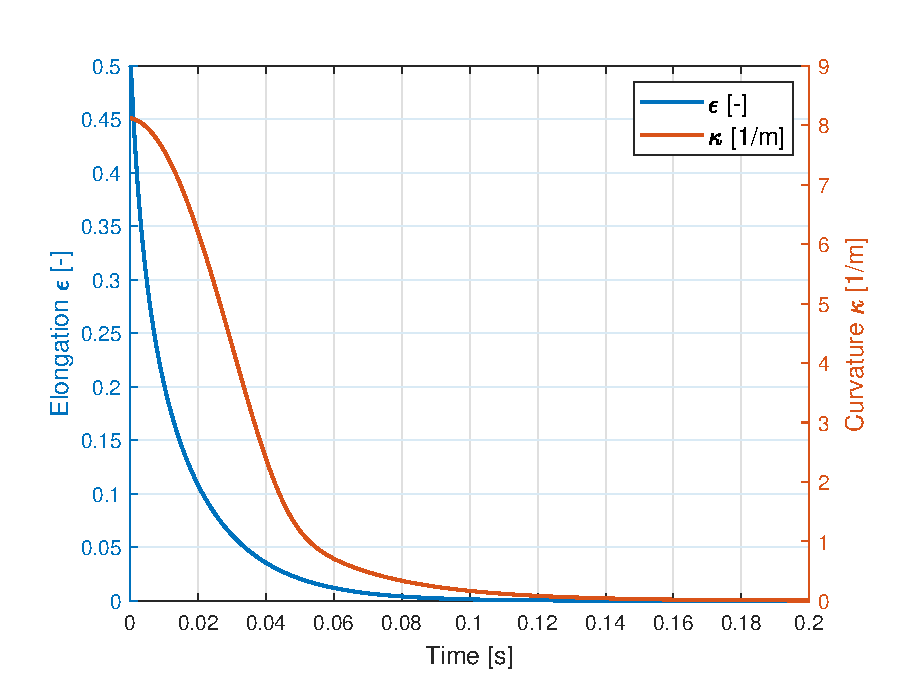
\includegraphics[width = \textwidth]{Figures/Chapter4/freeoschighd.eps}
    \caption{Free oscillation of the dynamic model with $q_0 = [8,0.5]$ for relatively high damping}
    \label{figapp4:highd}
    \end{minipage}
\begin{minipage}{0.48\textwidth}
    \centering
    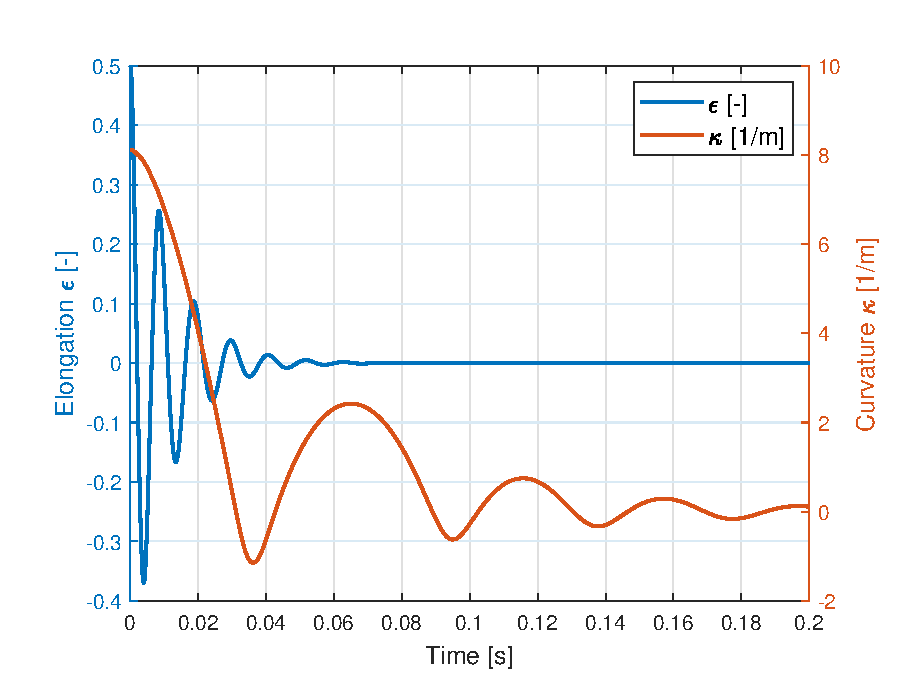
\includegraphics[width = \textwidth]{Figures/Chapter4/freeosclowd.eps}
    \caption{Free oscillation of the dynamic model with $q_0 = [8,0.5]$ for relatively low damping}
    \label{figapp4:lowd}
    \end{minipage}
\end{figure}